% Diese Zeile bitte -nicht- aendern.
\documentclass[course=asp]{aspdoc}

%%%%%%%%%%%%%%%%%%%%%%%%%%%%%%%%%
%% TODO: Ersetzen Sie in den folgenden Zeilen die entsprechenden -Texte-
%% mit den richtigen Werten.
\newcommand{\theGroup}{130} % Beispiel: 42
\newcommand{\theNumber}{A220} % Beispiel: A123
\author{Jeremy Immanuel \and Haskel Nisai}
\date{Wintersemester 2023/24} % Beispiel: Wintersemester 2019/20
%%%%%%%%%%%%%%%%%%%%%%%%%%%%%%%%%

% Diese Zeile bitte -nicht- aendern.
\title{Gruppe \theGroup{} -- Abgabe zu Aufgabe \theNumber}

\begin{document}
\maketitle

\section{Einleitung}
Wir haben vielleicht schon ein Bild eines CT-Scans oder BW-Filters in Instagram gesehen. Dies sind einige der Beispiele, bei denen Graustufen auf einem Bild verwendet werden. Graustufenbilder können je nach Kontext unterschiedliche Vorteile haben. Für die Ästhetik gibt es uns den klassischen 1950-Fotografie-Look zu unserem Bild, was es interessanter macht, daher wird es normalerweise als einer der Filter in der Fotobearbeitungs-App verwendet. In professionellen Bereichen werden Graustufen eingesetzt, um die Bildverarbeitung einfacher und effizienter zu gestalten und zu erkennen. In der Medizinwelt zum Beispiel verwenden CT-Scans grau skalierte Bilder, um die Analyse der Organe und des Gewebes durch den Arzt viel einfacher zu machen, mit weniger Ablenkung oder Verwirrung von Farben. In der Bildverarbeitung werden Graustufen zu Bildern implementiert, um die Komplexität des Algorithmus zu reduzieren und so die Berechnungskosten in Zeit und Rechenleistung zu senken.

Mit den Vorteilen der Grauskalierungstechnik ist es gerade für uns als Studierende der Fakultät Informatik am besten zu lernen, wie man sie effizient umsetzt, was ja das Ziel diese Ausarbeitung ist. Als Produkt wird ein kleines Graustufenprogramm entwickelt. Das Programm nimmt das Eingabebild im ppm-Format und gibt eine grau skalierte Version im pgm-Format zurück. Das resultierende Bild ist komplett mit Rauschenreduktion.

Im Laufe der Seiten werden verschiedene Lösungsansätze analysiert. Die Analyse umfasst die Korrektheit sowie die Leistung und den Vergleich zwischen den einzelnen Implementierungen. Dies stellt sicher, dass nicht nur die Graustufungsfunktion wie erwartet funktioniert, sondern das gesamte Programm auch robust und effizient ist.

%Losungsansatz%%%%%%%%%%%%%%%%%%%%%%%%%%%%%%%%%%%%%%%%%%%%%%%%%%%%%%%%%%%%%%%%%%%%%%%%%%%%%%%%%%%%%%%%%%%%%%%%%%%%%%%%%%%

\section{Lösungsansatz}
\subsection{Beobachtungen und Erkenntnisse}
Wenn wir uns ein grau skaliertes Bild ansehen, stellen wir fest, dass das gesamte Bild nur im Schwarzton dargestellt wird. Das bedeutet, dass jeder einzelne farbige Pixel später nur noch eine Farbe im Schwarzton annimmt. Dazu müssen wir in der Lage sein, jeden Pixel im gesamten Bild zu manipulieren.
Manchmal kann eine Farbmanipulation in einem Bild Geräusche verursachen. Diese Geräusche lassen das Bild körnig und manchmal sogar komplett ausgeformt aussehen. Um dies zu vermeiden, wird die Rauschunterdrückung auf das Bild angewendet. Die Rauschunterdrückung besteht aus Laplace-Filterung und Weichfokussierung/-zeichnung. Laplace-Filter ist die Methode, um Kanten in einem Bild zu erkennen. "The Laplacian of an image highlights regions of rapid intensity change and is an example of a second order or a second derivative method of enhancement. It is particularly good at finding the fine details of an image. Any feature with a sharp discontinuity will be enhanced by a Laplacian operator" \cite{satu}.Weichzeichnung ist die Technik, ein Foto oder einen Film etwas unklar erscheinen zu lassen, um ihm einen romantischen Effekt zu verleihen\cite{mw:abulia}.

\subsection{Konzeptioneller Lösungsansatz der Entwicklung einer Graustufungsfunktion}
Nach dem Ergebnis der ppm-Konvertierungsfunktion können wir ein flaches Array von unsignierten 8-bit Ganzzahlen verwenden, um jedes Pixel aus unserem manipulierbaren Bild darzustellen. Als nächstes müssen wir unser farbiges Pixel in einen Schwarzton verwandeln. Eine Farbe wird in einem Schwarzton sein, wenn R,G und B-Werte denselben Wert annehmen. Wir können unsere RGB-Werte in einen Wert umrechnen und Konstanten hinzufügen, um den Einfluss jedes R-, G- und B-Kanals in der Berechnung zu kontrollieren.

Sowohl der Laplace-Filter als auch der Softfocus verwenden eine Faltungsmatrix bei der Berechnung. In der Faltungsmatrix-Formel müssen wir in der Lage sein, ein Pixel basierend auf spezifiziertem x und y zu erhalten. In der Implementierung wird eine Funktion namens "getPixelAt" dies tun.

%Algorithmischen Ansatz%%%%%%%%%%%%%%%%%%%%%%%%%%%%%%%%%%%%%%%%%%%%%%%%%%%%%%%%%%%%%%%%%%%%%%%%%%%%%%%%%%%%%%%%%%

\subsection{Algorithmische Ansätze und ihre Implementierungen zur Graustufung eines Bildes }
\subsubsection{Ansatz 1 - naive C Implementierung}
Die erste Umsetzung folgt naiv der oben beschriebenen Abstraktion. Zuerst nehmen wir die angegebene ppm-Bilddatei, die der Benutzer als Eingabe eingegeben hat, und konvertieren sie in ein Array von vorzeichenlosen 8-Bit-Ganzzahlen. Dann verfärben wir das Bild mit der Graustufenfunktion. Dann implementieren wir die eigentliche Denoise, die aus dem Laplace-Filter und dem Soft Focus besteht. Aber um der Funktionsbenennung im Aufgabenblatt zu folgen, rufen wir die Entfärbung, den Laplace-Filter und den Weichzeichner von einer Funktion auf, die wir in diesem Fall als Denoise bezeichnen. Während der Berechnung rufen wir eine Funktion namens "getPixelAt" auf, um das Pixel im Flatten-Array basierend auf dem angegebenen x und y zu erhalten.
Nachdem alle Berechnungen abgeschlossen sind, geben wir sie in der angegebenen Ausgabedatei im pgm-Format aus. Um diese Implementierung zu verwenden, führen Sie das Programm mit der Option -V 3 aus
\\
\\*
\texttt{./gogrey -V 3}

\subsubsection{Ansatz 2 - optimierte C Implementierung}
Wir können die erste Implementierung optimieren, indem wir etwas Padding im Flat Array hinzufügen. Das Padding hilft, redundante Randchecks im "getPixelAt" zu vermeiden und somit die Laufzeit zu verbessern. Wir tauschen einen geringen Speicherplatz gegen eine erhebliche Leistungsoptimierung aus. Folglich müssen die folgenden 2 Bedingungen erfüllt sein:
\begin{itemize}
    \item Die Differenzen der vertikalen Pixelindexes (angenommen, dass das Pixelarray zu 2-dimensionalem Array geordnet wird) müssen konstant sein. Die Differenzen der horizontalen Pixelindexes müssen natürlich ebenfalls eins bleiben.
    \item Für jedes Pixel, das kein Padding ist, müssen Nachbarn (vertikal, horizontal und diagonal) vorhanden sein, auf die zugegriffen werden kann. Also, die Nachbarn dürfen nicht NULL sein.
\end{itemize}

\begin{figure}[h]
    \centering
    \includegraphics[width=3.2cm]{graphics/padded array 1.png}
    \quad
    \includegraphics[width=3.2cm]{graphics/padded array 2.png}
    \caption{Beispiel von Padded Array}
    \label{fig:my_label}
\end{figure}

Der Speicherbereich des Padding wird vernachlässigt und die Anzahl der Padding wird mit zunehmender Größe des Bildes proportional kleiner. Sie können das Programm mit dieser Implementierung ausführen, indem Sie die Option -V 2 hinzufügen.\\
\\*
\texttt{./gogrey -V 2}\\
\\*

\subsubsection{Ansatz 3 - Assembly Implementierung}
Die ASM-Implementierung wurde Zeile für Zeile aus der optimierten C Implementierung übersetzt. Dabei wurden die Iterationen an die selben algorithmischen Ansätze angelehnt, wie in der C Implementierung. Für diese Version wurden jedoch keine weiteren Optimierungsmöglichkeiten festgestellt. Sie können das Programm mit dieser Implementierung ausführen, indem Sie die Option -V 1 hinzufügen.\\
\\*
\texttt{./gogrey -V 1}\\

\subsubsection{Ansatz 4 - Assembly Implementierung mit SIMD optimierung}
Der vierte Ansatz, die SIMD Implementierung, hält sich an die ASM Implementierung, nutzt jedoch SIMD Register. Diese Implementierung ist unsere Hauptimplementierung und wird standardmäßig verwendet, wenn beim Starten des Programms keine Versionsoption angegeben wird. Um das Programm mit dieser Implementierung auszuführen, fügen Sie entweder die Option -V 0 hinzu oder geben Sie keine Version an.\\
\\*
\texttt{./gogrey -V 0}\\

%Korrektheit%%%%%%%%%%%%%%%%%%%%%%%%%%%%%%%%%%%%%%%%%%%%%%%%%%%%%%%%%%%%%%%%%%%%%%%%%%%%%%%%%%%%%%%%%%%%%%%%%%%%%%%%%

% TODO: Je nach Aufgabenstellung einen der Begriffe wählen
\section{Genauigkeit}
Es stellt sich die Frage, ob die Konstruktion der Grauskalierung sowie des Programms aufgrund des gewählten konzeptionellen Ansatzes sowie der algorithmischen Ansätze der Implementierungen klar ist. Dies wird in diesem Kapitel untersucht. Hier werden wir über die Kriterien sprechen, die verwendet werden, um zu bestimmen, ob die Grauskalierung richtig funktioniert. Anschließend wird die Korrektheit der Implementierung analysiert und bewertet. Darüber hinaus wird auch die Robustheit des Programms überprüft. Auf diese Weise stellen wir sicher, dass das angegebene Programm nicht nur korrekt, sondern auch genau ist.

\subsection{Kriterien für eine korrekte Graustufenumsetzung}
Wir können anhand dieser Elemente feststellen, ob die Grauskalierung korrekt durchgeführt wurde.

\begin{enumerate}
\item Das Ausgabebild besteht nur aus Farben im Schwarzton.
\item Das Ändern von Gewichtskonstanten ändert auch das Ausgabebild.
\item Ein Bild, das bearbeitet wird (zum Beispiel in Helligkeit oder Farbton und Sättigung), gibt ein anderes Graustufenbild aus als die nicht bearbeitete Version.
\item Alle Objekte im Bild sind deutlich zu sehen. Aufgrund der fehlenden Kantenerkennung im Laplace-Filter verschmelzen keine Objekte miteinander.
\item Keine Artefakte im Ausgabebild. Falsche Berechnung, versehentliches Umschalten in x- und y-Achse sowie Überläufe können Artefakte im Ausgabebild verursachen.
\end{enumerate}

\subsection{Korrektheit der Implementierung der Grauskalierung}
Jetzt werden wir die Korrektheit der von uns erstellten Grauskalierungsfunktion testen. Wir haben einige Bilder zum Testen von Punkt 1, 3, 4 und 5 bereitgestellt.
\begin{itemize}
    \item Bilder im Hoch- und Querformat.
    \item Ein Originalbild und eine bearbeitete Version dieses Bildes.
    \item Bild mit verschiedenen Farben, das den gleichen gemittelten RGB-Wert hat.
\end{itemize}
Um Punkt 2 zu testen, führen wir das Programm zuerst im Standardmodus aus. Danach werden randomisierte Koeffizienten für a, b und c verwendet. Wir werden den randomisierten Lauf fünfmal wiederholen, um sicherzustellen, dass alles tatsächlich anders ist.\\
\\*
\texttt{./gogrey.exe} \\

dann führen wir diesen Code unten für 5 mal aus\\\\
\texttt{./gogrey.exe --coeffs <random a, random b, random c>} \\
\\
Der Test wird an unserer Hauptimplementierung sowie an der optimierten C-Implementierung durchgeführt. Die Ausgaben aller oben genannten Testelemente sind wie folgt. Die Reihenfolge der Bilder von links nach rechts sind : Eingabebild, Ausgabe von Hauptimplementierung, Ausgabe von C mit Padding.
\begin{figure}[h]
    \centering
    \includegraphics[width=3.2cm]{graphics/rgbcolor.png}
    \quad
    \includegraphics[width=3.2cm]{graphics/rgb.png}
    \quad
    \includegraphics[width=3.2cm]{graphics/rgbC.png}
    \caption{Beispiel aus einem Bild mit verschiedenen Objekten unterschiedlicher Farbe, aber gleichen durchschnittlichen RGB-Wert}
    \label{fig:my_label}
\end{figure}

\begin{figure}[h]
    \centering
    \includegraphics[width=3.2cm]{graphics/oricolor.JPG}
    \quad
    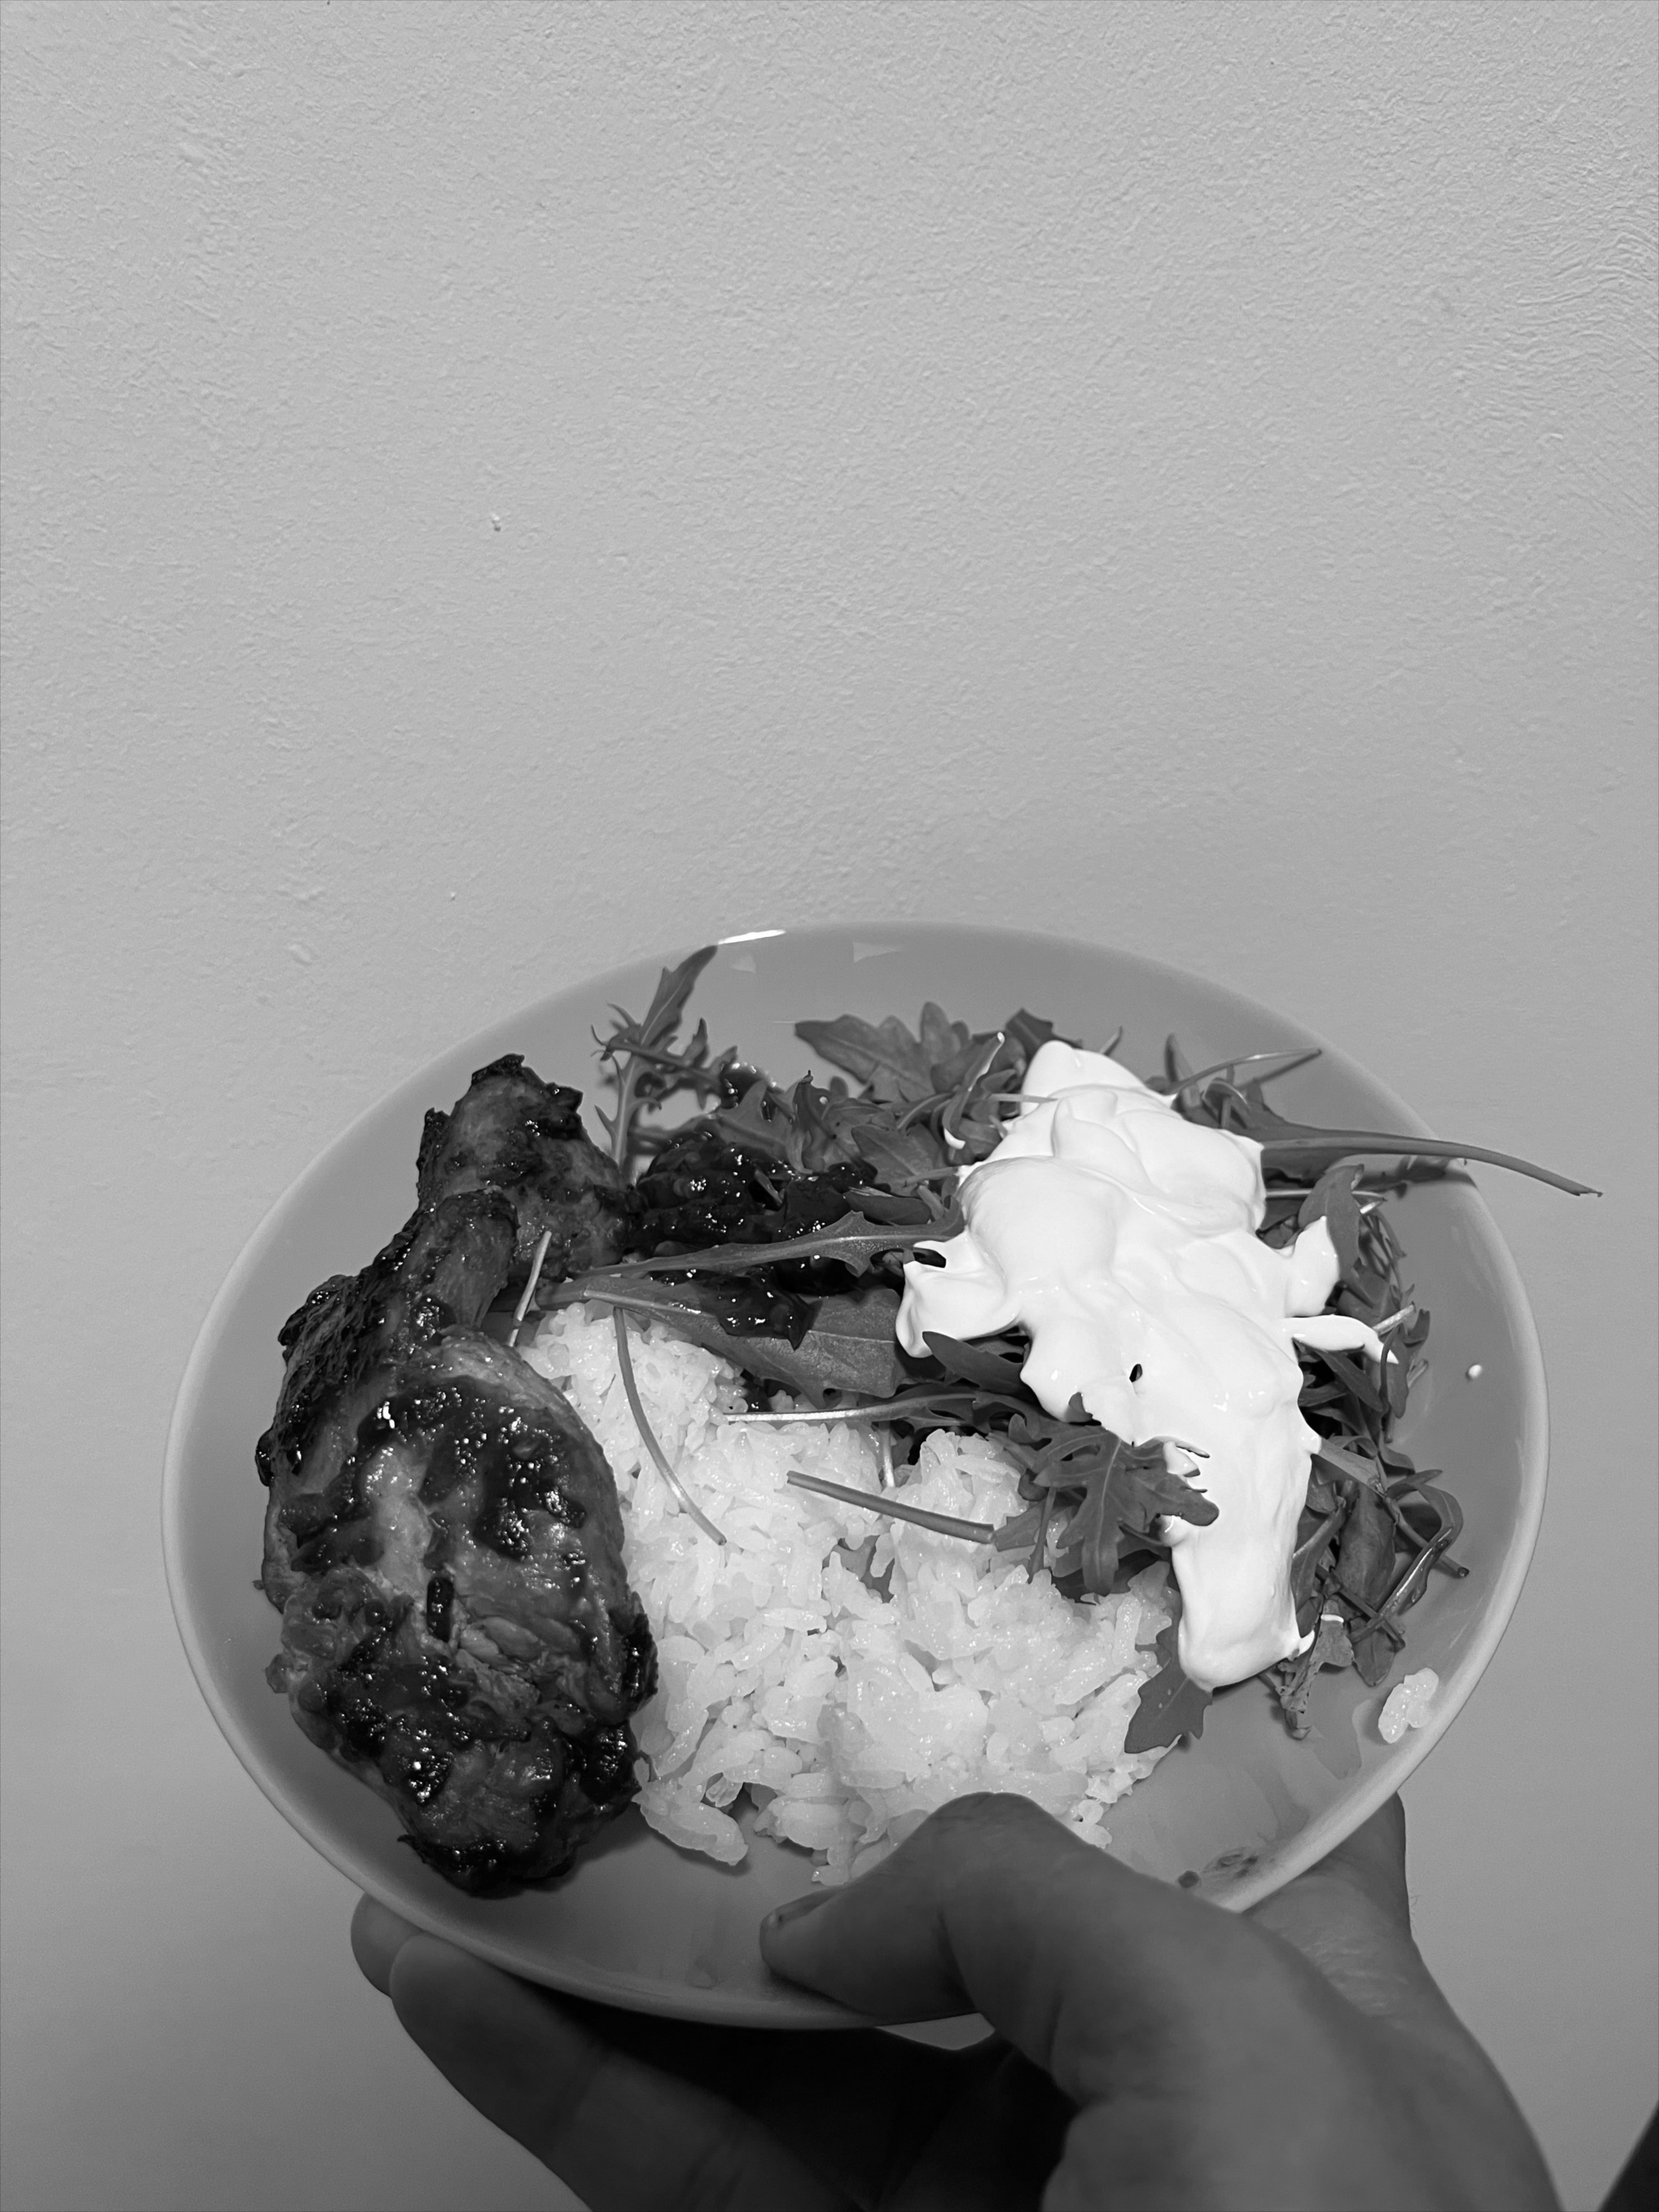
\includegraphics[width=3.2cm]{graphics/ori.png}
    \quad
    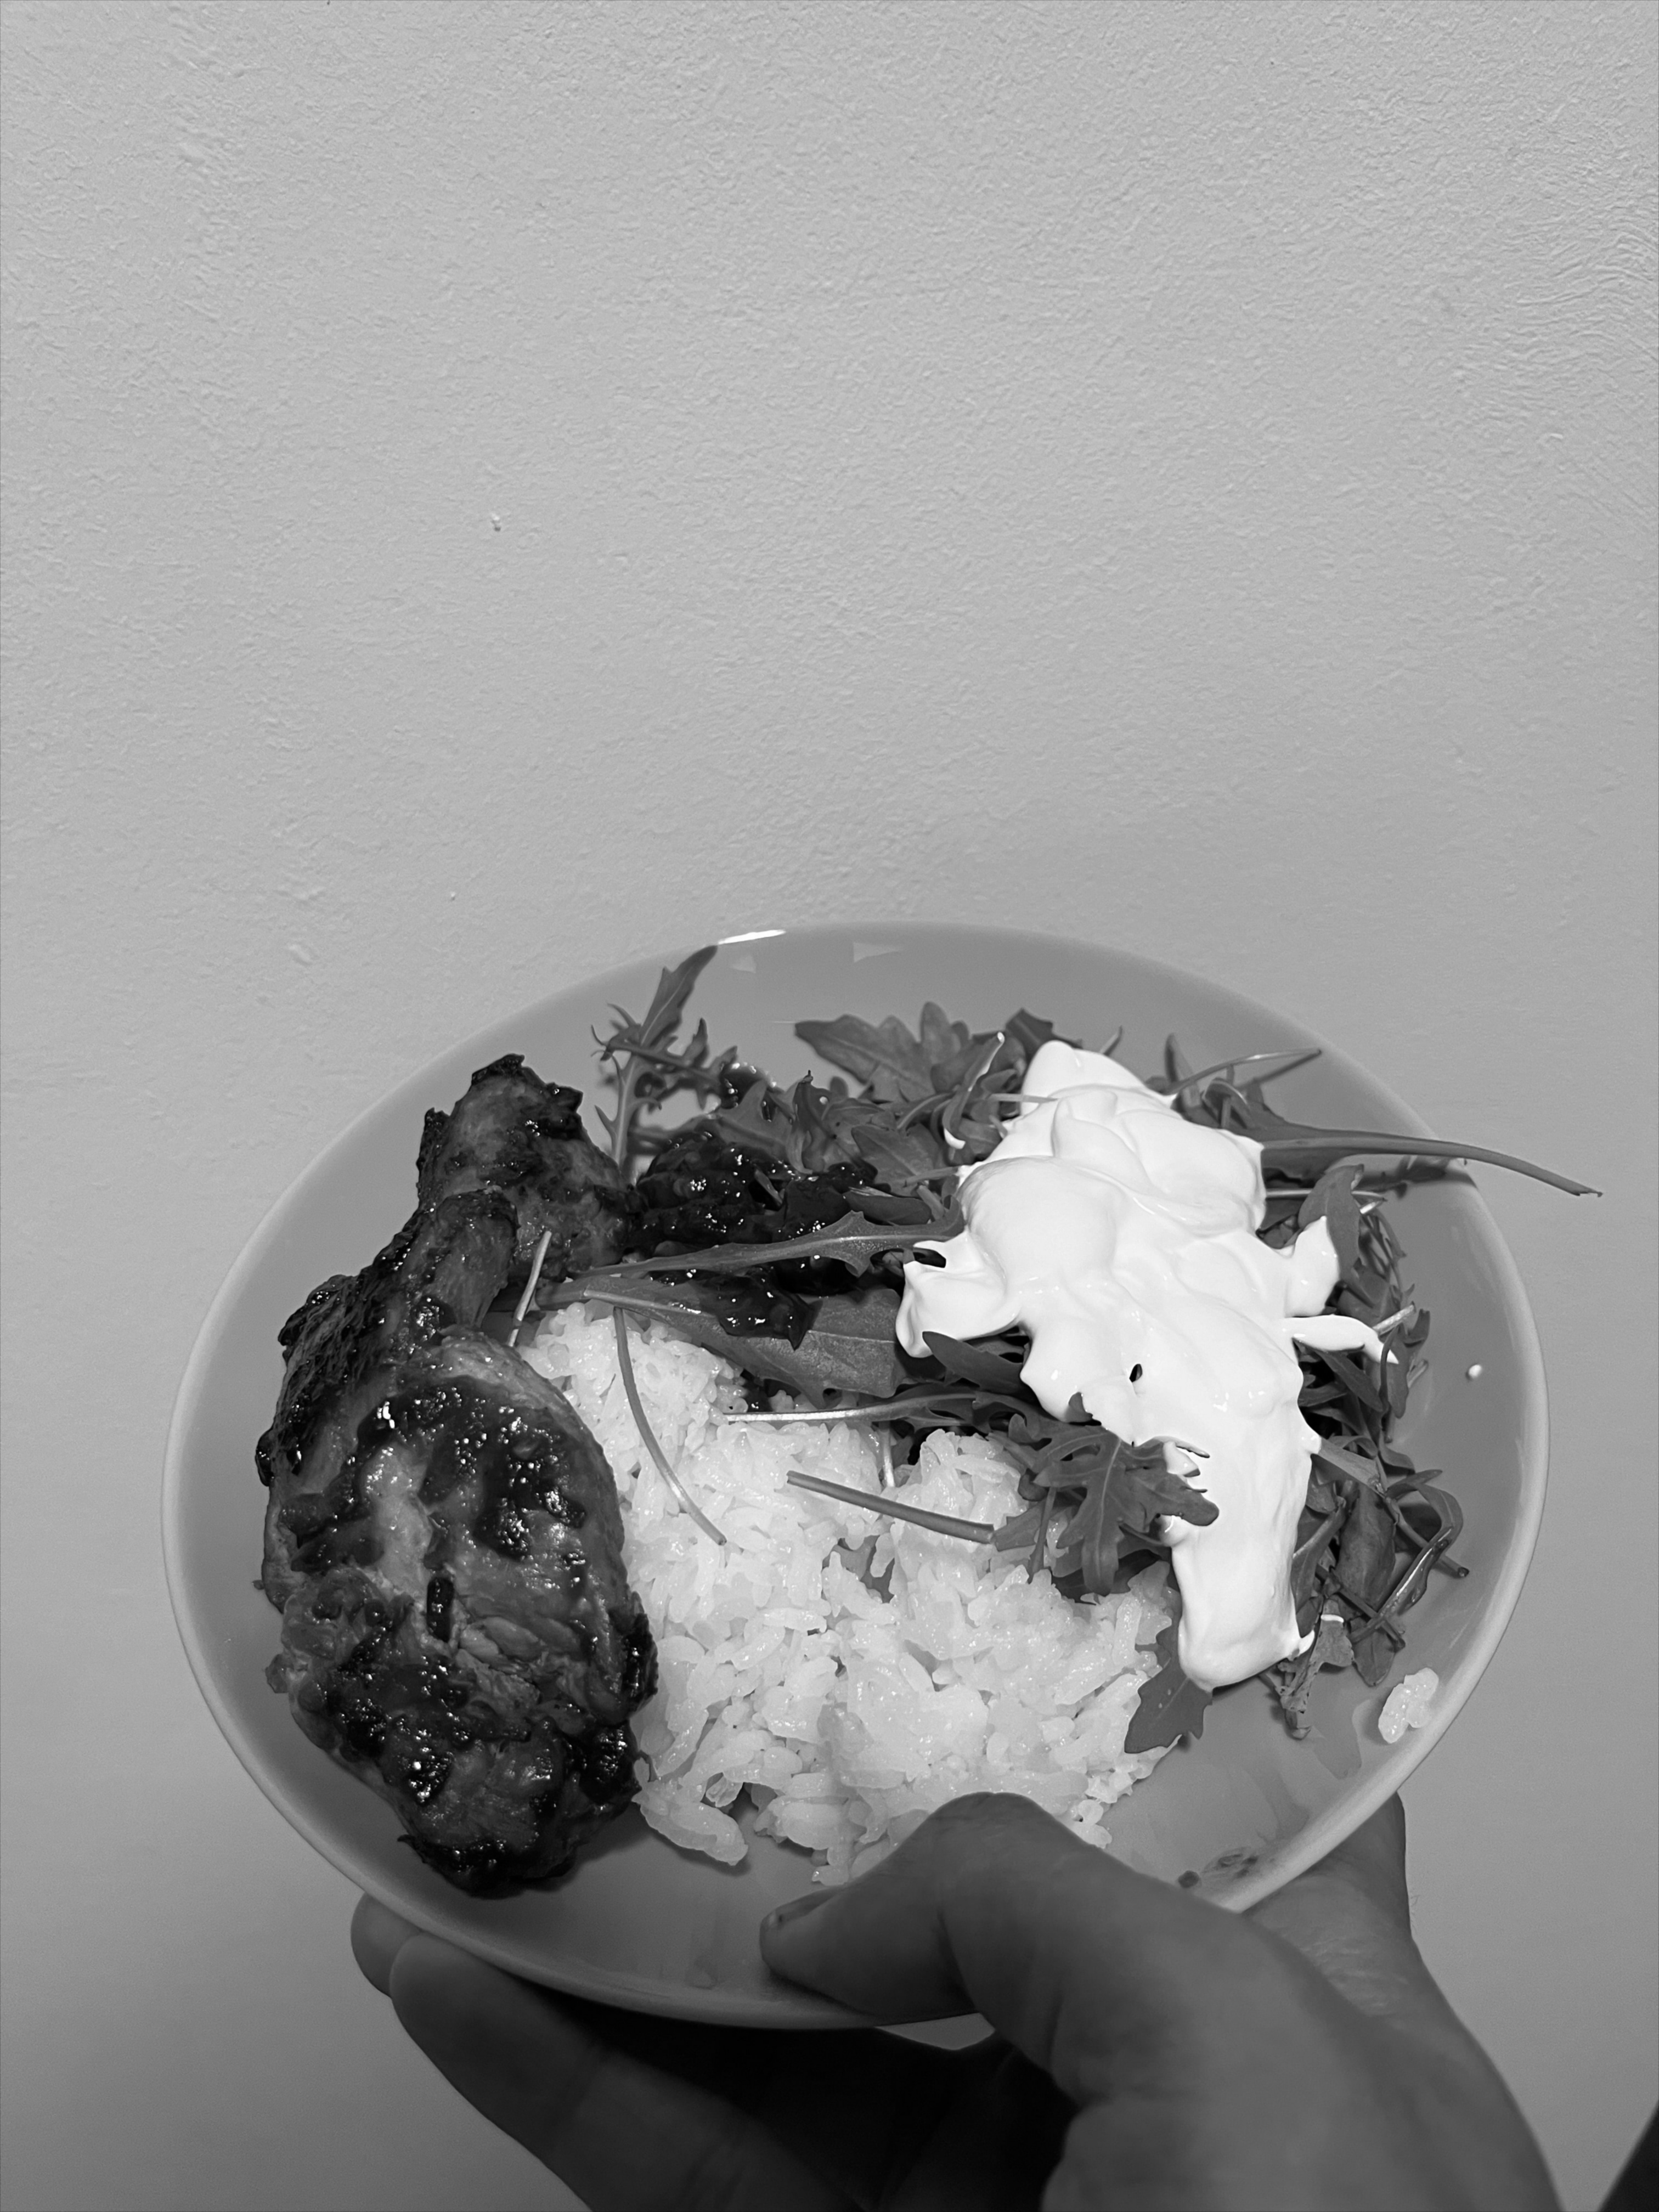
\includegraphics[width=3.2cm]{graphics/oriC.png}
    \caption{Originalbild}
    \label{fig:my_label}
\end{figure}

\begin{figure}[h]
    \centering
    \includegraphics[width=3.2cm]{graphics/editcolor.jpg}
    \quad
    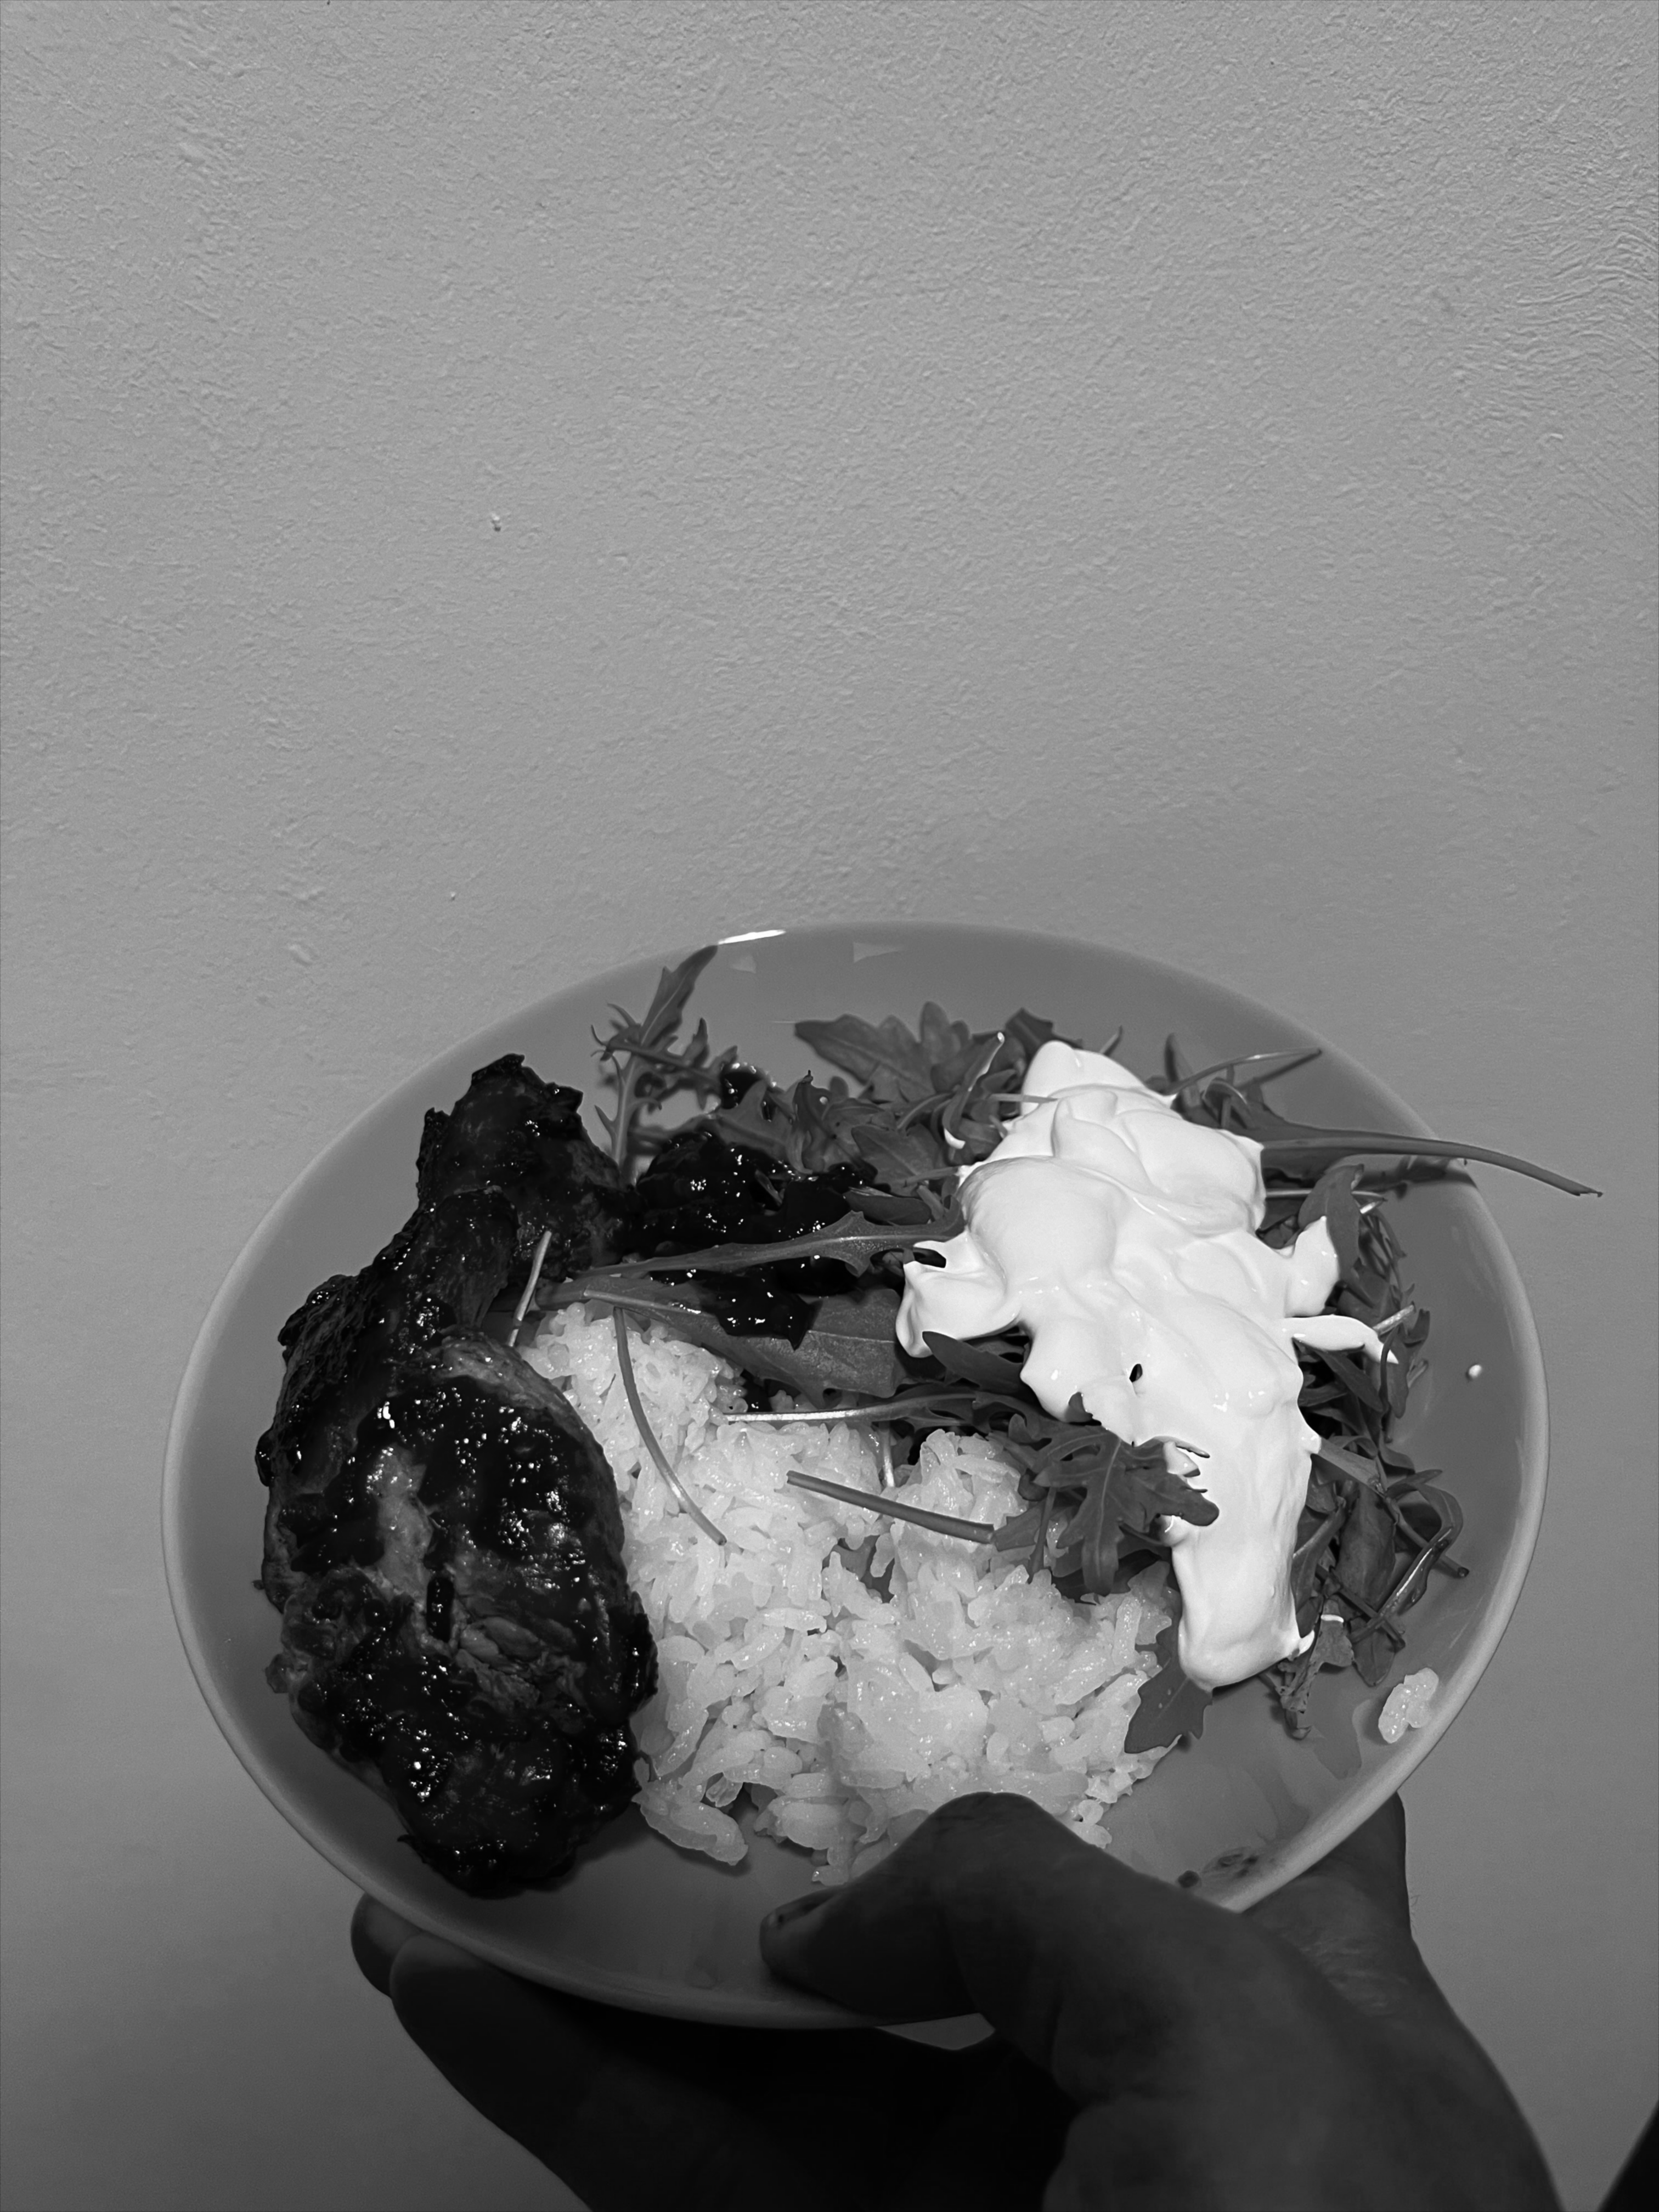
\includegraphics[width=3.2cm]{graphics/edit.png}
    \quad
    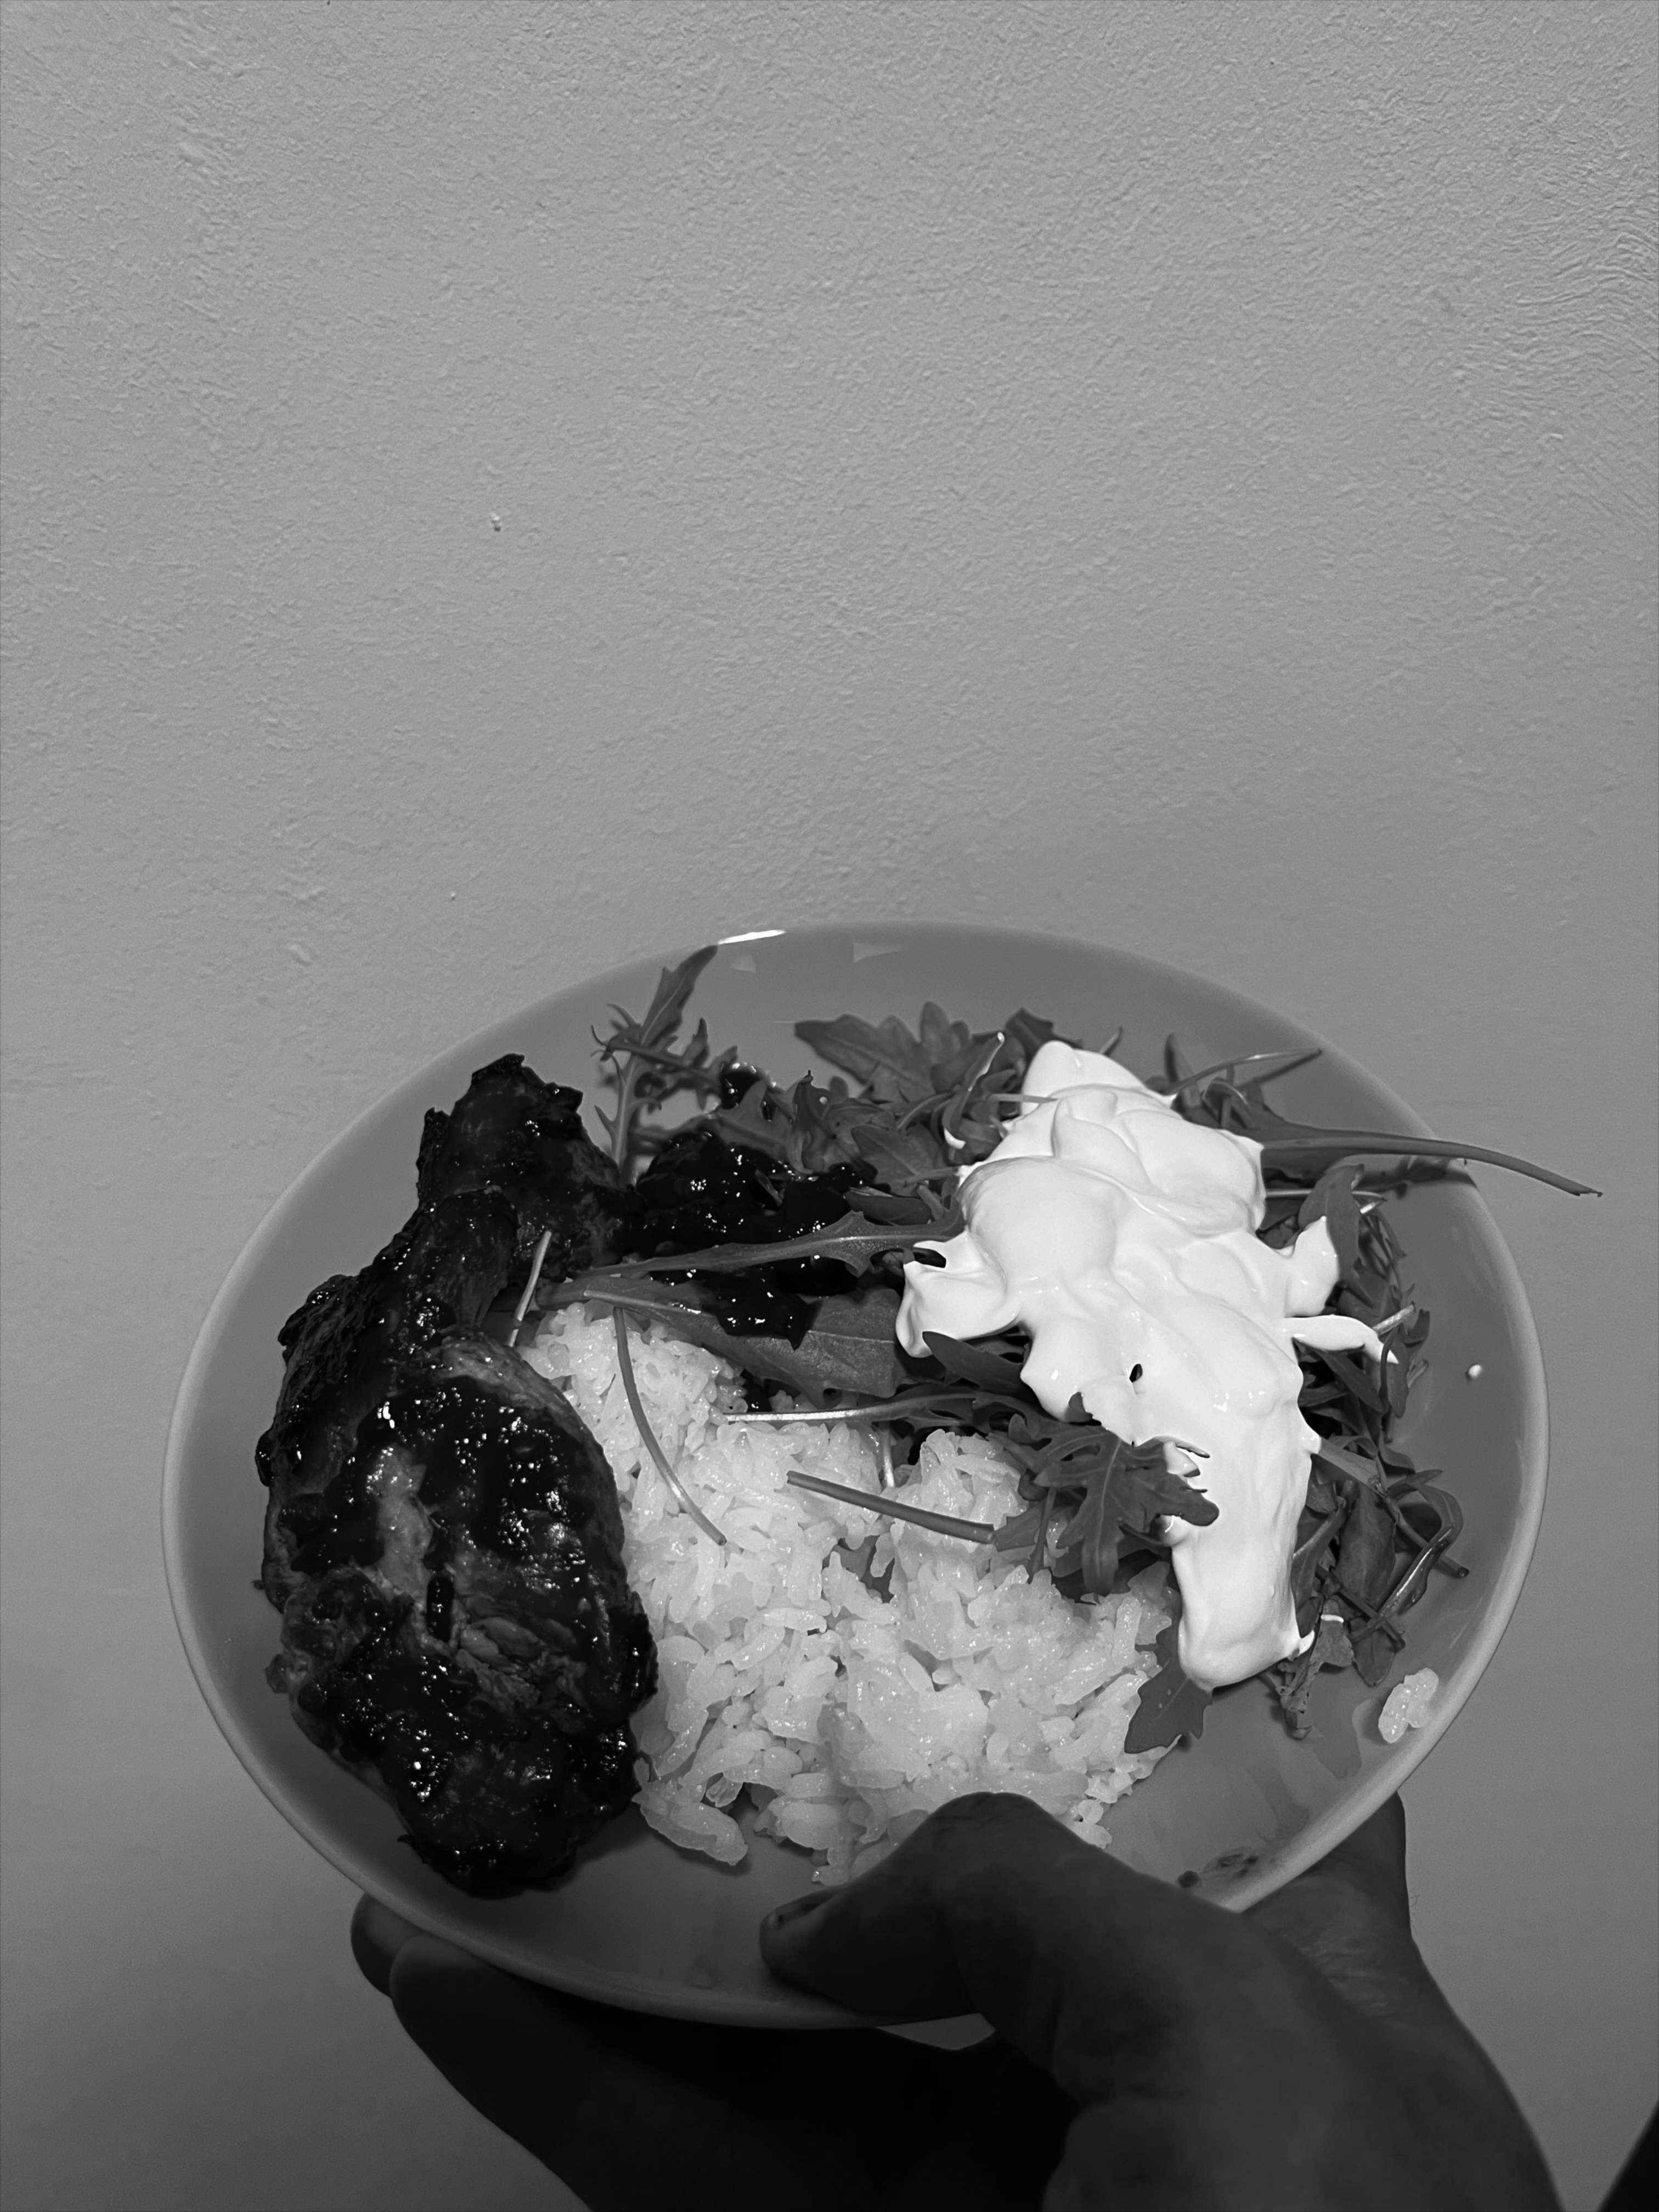
\includegraphics[width=3.2cm]{graphics/editC.png}
    \caption{Bearbeitetes Bild aus Abbildung 3. Helligkeit und Sättigung wurde geändert}
    \label{fig:my_label}
\end{figure}

\begin{enumerate}
    \item Enthalten alle Ausgabebilder nur Farben im Schwarzton?\\Ja.
    \item Hat ein bearbeitetes Bild eine andere Ausgabe als das Original?Ja, können wir im Abschnitt 3 sehen.
    \item Sind alle Objekte im Bild deutlich zu sehen?\\Ja, Abschnitt 3 zeigt, dass die benachbarten Pixel mit dem gleichen gemittelten RGB-Wert immer noch getrennt sind.
    \item Gibt es irgendwelche Artefakte in den resultierenden Bildern?\\Nein, alle Ausgaben entsprechen perfekt ihren Eingaben.
\end{enumerate}

\subsection{Eindeutigkeit des Programms}
Unerwartet Eingaben werden ebenfalls im Rahmenprogramm noch vor Beginn der Berechnung abgefangen, sodass es zu keinen fehlerhaften Ergebnissen kommt. Aufrufe mit beispielsweise einem übergebenen Dateinamen, welcher für die SVG-Erstellung unvorteilhaft ist werden frühzeitig erkannt und abgebrochen.


\section{Performanzanalyse}
Die Leistungsanalyse konzentriert sich auf den Vergleich verschiedener algorithmischer Ansätze hinsichtlich ihrer Laufzeit für die Vervollständigung der Grauskalierung. Die Umsetzung wird nach einem spezifischen Verfahren analysiert und bewertet, das im Folgenden näher erläutert wird. Leistungskritische Optimierungen werden näher benannt, ihr Einfluss analysiert und begründet. Dazu werden die Implementierungen nach der Reihenfolge ihrer chronologischen Ableitung, wie im Lösungsansatz beschrieben, analysiert.

Für die Datenerfassung werden vier Testfälle erstellt. Testfälle basieren auf den Implementierungsvarianten. Jeder Testfall erhält 3 verschiedene Eingabebilder mit unterschiedlichen Größen: klein, mittel, groß, und sehr groß. Alle Bilder haben das gleiche Seitenverhältnis von 1:1. 1000 Tests werden für jede der Bildgrößen durchgeführt und die Zeit für die Berechnung wird dann gemittelt. Die für den Test verwendete Hardware ist ein Lenovo Legion 5 2020 Laptop mit 8-Core 16-Threads AMD Ryzen 7 4800H Prozessor und 16GB NVME RAM. kompiliert wurde mit Make(GCC 8.3.0), GNU17 Standard, Optimierungsstufe -O3. 

\subsection{Vorgehensweise der Performanzanalyse}
Zur Analyse der Performanz einzelner Implementierungen haben wir uns für die folgende Vorgehensweise entschieden.

\begin{enumerate}
    \item Implementierung einer asymptotischen Wachstumsrate und Durchschnittslaufzeit.
    \item Analyse der getroffenen oder nicht-getroffenen Optimierungen.
    \item Bewertung der Performanz jeder Implementierung.
\end{enumerate}

\subsection{Laufzeitmessungen}
Die gesamte Grauskalierungsfunktion wird als Denoise bezeichnet, wie das Aufgabenblatt vorschlägt. Die Laufzeitmessung wird unmittelbar vor dem Aufruf der Denoise gestartet und unmittelbar nach erfolgreichem Abschluss der Berechnung gestoppt. Die Input- und Output-Konvertierung zählt nicht zur Zeitmessung, da das Rahmenprogramm sie immer aufruft, unabhängig von der Implementierung.
Der arithmetische Mittelwert der Laufzeit in Sekunden wurde in der folgenden Tabelle eingetragen.

\begin{center}
    \begin{table}[ht]
        \centering
        \begin{tabular}{ |m{7em}|m{7em}|m{7em}|m{7em}|m{7em}| }
        \hline
        Bildgröße & Hauptimplementierung & Assembly ohne SIMD & Optimierte C Implementierung & Naive C Implementierung \\
        \hline
        \hline
            640x426 & 0.000368 & 0.004636 & 0.001324 & 0.002346\\ 
        \hline
            1280x853 & 0.001558 & 0.019114 & 0.005304 & 0.009543\\
        \hline
            1920x1280 & 0.003630 & 0.042802 & 0.011890 & 0.021478\\
        \hline
            5184x3456 & 0.026554 & 0.0.304948 & 0.086038 & 0.155976\\
        \end{tabular}
        \label{tab:Versionsunterschiede}
    \end{table}
\end{center}

\subsubsection{Laufzeit der naiven C Implementierung}
 Innerhalb Denoise werden die Entfärbungsfunktion, der Laplace-Filter und der Weichzeichner aufgerufen. 

Die Entfärbungsfunktion iteriert über jeden einzelnen Pixel im Bild und macht den Durchschnitt. Die Gesamtlaufzeit der Funktion ist O($w*h$), wobei h die Höhe und w die Breite ist. also die asymptotische Laufzeit der Funktion ist O($n$).

Sowohl Laplace-Filter als auch Soft Focus bestehen hauptsächlich aus Checks und einfacher Arithmetik, während sie durch jedes einzelne Pixel im Bild iterieren. Es scheint nicht viel, aber die Funktion ruft auch die getPixelAt-Funktion so oft pro Iteration auf. Dies wird interessanter, wenn wir zur Diskussion der Laufzeit aus der optimierten Version kommen. Die Gesamtlaufzeit der Funktion ist O($w*h$), wobei h die Höhe und w die Breite ist. Also ist die asymptotische Laufzeit die 2 Funktionen ist etwa O($2n$), n hier die Anzahl des Pixels im Bild.

Insgesamt ist die naive C-Laufzeit O($4w*h$) und asymptotisch ist sie O($n$)
Die Durchschnittslaufzeit der naiven C Implementierung in Sekunden beträgt: 

\subsubsection{Laufzeit der optimierten C Implementierung}
Je größer das Bild, desto geringer die zusätzliche Padding, die in der flachen Anordnung hinzugefügt wird, desto geringer ist also die Optimierung. Die in Bezug auf Größe x und y benötigte Padding kann wie folgt dargestellt werden ... .

Durch das Padding entfällt die Notwendigkeit, die Funktion "getPixelAt" aufzurufen, die in der naiven Implementierung in der Regel mehrmals pro Pixel ausgeführt wird. Wenn diese Funktion nicht aufgerufen wird, wird die Berechnung schneller ausgeführt. Dies liegt an der Entfernung mehrerer Funktionsaufrufe pro Pixel. obwohl die asymptotische Laufzeit immer noch O($n$) ist. Es ist aber interessant, das Die Gesamtlaufzeit der Funktion O($4w*h + padding$) ist, wobei h die Höhe und w die Breite ist.

Das optimierte C ist etwa 2 mal schneller als die normale Implementierung für ein Bild mit geringer Größe. Bei großen Bildern ist die optimierte C-Implementierung jedoch nur geringfügig schneller als die naive.

\subsubsection{Laufzeit der Assembly Implementierung}
Da die Assembly Implementierung auf dem algorithmischen Ansatz der optimierten C Implementierung basiert, kann auch hier die Laufzeitklasse O($n$) zugeordnet werden.

\subsubsection{Laufzeit der SIMD Assembly Implementierung}
Auch hier wird die Laufzeitklasse O($n$) zugeordnet.

\subsection{Analyse der getroffenen oder nicht-getroffenen Optimierungen}

\subsubsection{Optimierungen der naiven C Implementierung}
Was wir im zweiten Kapitel über die naive C-Implementierung vorher besprochen haben, gibt es nur wenige Optimierungen, die wir tun können. Die Laufzeit wird insbesondere durch häufiges Aufrufen der Funktion "getPixelAt" beeinflusst. Wie wir bereits zuvor festgestellt haben, wäre es ein Optimierungsansatz, ein gepolstertes Array zu erstellen.

\subsubsection{Optimierungen der optimierten C Implementierung}
Die oben genannten Optimierungsmöglichkeiten werden hier angewendet. Es werden nicht mehr mehrere "getPixelAt"-Funktionsaufrufe pro Pixel benötigt, und stattdessen verwenden wir jetzt einfache, wenn sonst überprüft  zeigt, dass es eine fast 2-fache Verbesserung in der Laufzeit gab. Diese Opmtimisierung wird jedoch im Verhältnis kleiner, je größer das Bild ist. Wie wir sehen können, macht die Optimierung nur etwa 1.. Ein Teil der naiven Umsetzung.

\subsubsection{Optimierungen der Assembly Implementierung}
Da die Assembly-Implementierung eng an die algorithmischen Ansätze der optimierten C-Implementierung anschließt, sind keine Optimierungen der Laufzeit zu erwarten. Interessant ist, dass Obwohl die Optimierungsstufe -O3, mit der das Programm kompiliert wurde, die Assembly Implementierung noch schneller ist. Diese -O3 Phase verwendet verschiedene Techniken wie Inlining, Loop-Optimierung usw. während der Kompilierung, um C-Code so effizient wie möglich zu optimieren.

\subsubsection{Optimierungen der SIMD Assembly Implementierung}
Ziel war es, die Berechnungen mit den SIMD-Registern zu beschleunigen. Es gibt einen klaren Unterschied in der durchschnittlichen Laufzeit zwischen den Assembly-Implementierungen mit und ohne die Verwendung von SIMD-Registern. Die SIMD-Registernutzung hatte Einfluss auf die Laufzeit und die Optimierung war erfolgreich.

\subsection{Bewertung der Performanz jeder Implementierung}

\subsubsection{Bewertung der naiven C Implementierung}
Zusammenfassend wird festgehalten, dass durch die zuvor erlangten Erkenntnisse des Lösungsansatzes, der Analyse der Korrektheit und zum Schluss der Analyse der Performanz die naive C Implementierung eine ganz nach dem konzeptionellem Lösungsansatz gerichtete Implementierung darstellt und beweist, dass das Konzept korrekt arbeitet, jedoch auch schnell ersichtlich macht, dass Optimierungsbedarf besteht und Berechnungen zusammengeführt werden können. Sie stellt eine gute Veranschaulichung der Überlegungen des Lösungsansatzes dar.

\subsubsection{Bewertung der optimierten C Implementierung}
Zusammenfassend wird festgehalten, dass durch die zuvor erlangten Erkenntnisse ersichtlich ist, dass die Optimierungsansätze etwa 2-fach verbessert haben. Die Optimierungen waren ein Erfolg und gleichzeitig ist die Übersichtlichkeit des Codes beibehalten worden. 

\subsubsection{Bewertung der Assembly Implementierung}
Durch die zuvor erlangten Erkenntnisse ist ersichtlich, dass eine Laufzeitoptimierung im Vergleich zur optimierten C Implementierung nicht zu erwarten war. Im Vergleich schneidet diese Implementierung besser ab als die naive C Implementierung und die optimierte C Implementierung. Die Laufzeit wird als durchaus vertretbar für eine Assembly Implementierung bewertet.

\subsubsection{Bewertung der SIMD Assembly Implementierung}
Es ist festzuhalten, dass die SIMD Implementierung keine neuen algorithmischen Ansätze bietet, jedoch die Assembly Implementierung in ihrer Laufzeit verbessert und somit in ihrer Performanz besser abschneidet, als die Assembly Implementierung.


\subsection{Ergebnisse der Performanzanalyse}
Zusammenfassend bietet die Assembly mit SIMD-Implementierung die schnellste Grauskalierungsfunktion. Die SIMD- und Assembly-Implementierungen bieten die interessante Einsicht, dass die SIMD-Registernutzung eine Laufzeitdifferenz zur normalen Assembly bietet. Während der Leistungsanalyse traten keine unerwarteten Fehler auf. Es kann jedoch nicht ausgeschlossen werden, dass ein Laufzeitunterschied für eine sehr hohe Anzahl von Iterationen sowie eine sehr hohe Bildgröße auftritt. Um weitere Leistungsunterschiede zu ermitteln, wäre eine andere Testumgebung von Vorteil. Für das betrachtete Umfeld sticht Assembly mit SIMD jedoch als klarer Sieger hervor.

\section{Zusammenfassung und Ausblick}
Zu Beginn dieser Ausarbeitung wurde das Problem erläutert, warum Grauskalierung nutztlich ist und warum ein effizienter Code zur Entwicklung eines Grauskalierungprograms notwendig ist. Im Laufe der Ausarbeitung wurden Ansätze zunächst graphisch, daraufhin mathematisch dargestellt und zum Schluss wurden diese implementiert. Die Korrektheit der Ansätze wurde analysiert und bestätigt. Zum Schluss wurde die Performanz der unterschiedlichen Implementierungen untersucht und verschiedene Optimierungsansätze bewertet. Es hat sich herauskristallisiert, dass alle Lösungsansätze korrekt sind, jedoch werden nicht mehrere Lösungsansätze benötigt, um Bilder effizient zu verarbeiten, sondern nur ein effizienter Lösungsansatz. Die Assembly Implementierung mit SIMD Optimierung stellte sich als schnellste Implementierung dar. 

% TODO: Fuegen Sie Ihre Quellen der Datei Ausarbeitung.bib hinzu
% Referenzieren Sie diese dann mit \cite{}.
% Beispiel: CR2 ist ein Register der x86-Architektur~\cite{intel2017man}.
\bibliographystyle{plain}
\bibliography{Ausarbeitung}{}

\end{document}
